\documentclass[a4paper,10pt]{article}
\usepackage[a4paper, total={6in, 8in}]{geometry}
\usepackage[utf8]{inputenc}
\usepackage{graphicx} 
\setlength\parindent{0pt}
\begin{document}

\begin{titlepage}
	\centering
	
\includegraphics[width=.6\textwidth]{liu-logo.png}\par
	\vfill
	{\scshape\Large TDDC17 ARTIFICIAL INTELLIGENCE\par}
	{\huge\bfseries Lab 2: Search\par}
	\vspace{1cm}
	{\large\itshape Robin Andersson (roban591) \\ Lawrence Thanakumar Rajappa (lawra776)\par}
	\vfill
	{\large \today\par}
\end{titlepage}

\textbf{1. In the vacuum cleaner domain in part 1, what were the states and actions? 
What is the branching factor?}

The states are represented by GridPos which in turn is represented by the x and y position of a tile in the world.
This GridPos can then either represent a clean or a dirty tile.
The actions that can be performed are: suck dirt and move east, west, south and north.
The actions give that the branching factor is five.
\\ \\
\textbf{2. What is the difference between Breadth First Search and Uniform Cost Search in a domain where the cost of each action is 1?}

Since the cost of each action is 1, then the prioritization of the action with the lowest cost of Uniform-Cost Search will
give be same as the nearest action that Breadth First Search gives.
This means that there is no difference between the two.
\\ \\
\textbf{3. Suppose that $h1$ and $h2$ are admissible heuristics (used in for example A*). Which of the following are also admissible?
\\ a) $(h1+h2)/2$
\\ b) $2h1$
\\ c) $\max(h1,h2)$}

a) This is just the mean of $h1$ and $h2$ which means that it will never exceed $\max(h1, h2)$.
This is obviously admissible since $h1$ and $h2$ are both admissible, meaning that the mean must be less than the true cost.
\\
b) This is not admissible since $2h1$ can exceed $\max(h1, h2)$ which means that it also can exceed the true cost.
\\
c) As explained in a) this is admissible since it cannot exceed $h1$ or $h2$ and since both of those are admissible then
this heuristics must also be less than the true cost.
\\ \\
\textbf{4. If one would use A* to search for a path to one specific square in the vacuum domain, what could the heuristic $(h)$ be? The cost function $(g)$? Is it an admissible heuristic?}

A heuristic could be the straight-line distance, since it cannot be overestimated. 
The cost function could be the one for each action that must be performed to reach the goal tile from the initial tile.
Thus the heuristic can never exceed the cost function since the straigh-line distance is the shortest path between to tiles, meaning that the heuristic is admissible.
\\ \\
\textbf{5. Draw and explain. 
Choose your three favorite search algorithms and apply them to any problem domain (it might be a good idea to use a domain where you can identify a good heuristic function). 
Draw the search tree for them, and explain how they proceed in the searching. 
Also include the memory usage. 
You can attach a hand-made drawing.}

\begin{figure}[ht]
	\centering
	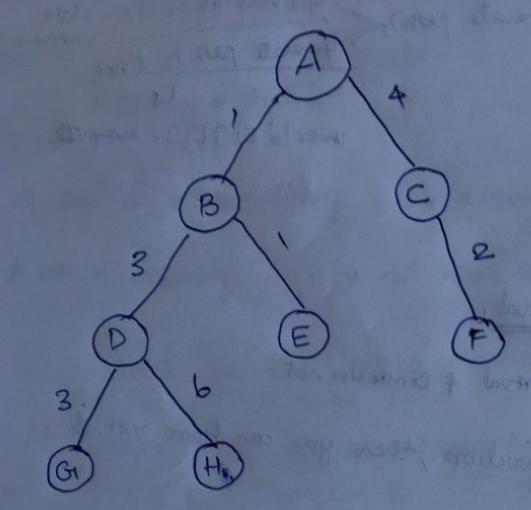
\includegraphics[width=.4\textwidth]{graph.png}
	\caption{The graph used to compare BFS, DFS and UCS.}
\end{figure}

Breadth-first search
\begin{itemize}
	\item Memory usage: it needs to remember every node on each level.
	\item The path explored is: $A \rightarrow B \rightarrow C \rightarrow D 
	\rightarrow E \rightarrow F \rightarrow G \rightarrow H$
\end{itemize}

Depth-first search
\begin{itemize}
	\item Memory usage: it needs to remember one node on each level.
	\item The path explored is: $A \rightarrow B \rightarrow D \rightarrow G \rightarrow 
	H \rightarrow E \rightarrow C \rightarrow F$
\end{itemize}

Uniform-cost search
\begin{itemize}
	\item Memory usage: it needs to remember every node on each level.
	\item The path explored is: $A \rightarrow B \rightarrow E \rightarrow D \rightarrow 
	C \rightarrow F \rightarrow G \rightarrow H$
\end{itemize}

\textbf{6. Look at all the offline search algorithms presented in chapter 3 plus A* search. 
Are they complete? Are they optimal? Explain why!}

\begin{enumerate}
	\item \textbf{Breadth First Search:} 
	It is complete, if the number of nodes is finite and it will also visit all the nodes and 
	will find the solution. But it is only optimal if the cost for each step is the same.
	\item \textbf{Uniform Cost Search:} 
	It is based on BFS. It is both complete and optimal. 
	It uses a priority queue instead of a FIFO queue.
	\item \textbf{Depth First Search:} 
	DFS is not complete as it will infinitely loop on a branch. 
	Moreover, it will return the first found solution, even when a lower-cost solution exists.
	Hence it is not optimal.
	\item \textbf{Depth limited search:} 
	The main goal of this algorithm is to reduce the depth to solve the infinite path problem, 
	but if the goal is situated beyond the limit, then this algorithm will not return the solution. 
	Hence it is not complete and it is not optimal for the same reason as DFS.
	\item \textbf{Bidirectional:} 
	Bidirectional search is complete if BFS is used in both searches. 
	It is optimal if BFS is used for search and the paths have uniform cost.
	\item \textbf{Iterative Deepening Depth First Search:} 
	Like BFS it is complete if the branching factor $b$ is finite and it is optimal if the 
	step cost is the same.
\end{enumerate}

\textbf{7. Assume that you had to go back and do Lab 1/Task 2 once more 
(if you did not use search already). 
Remember that the agent did not have perfect knowledge of the environment but had to explore 
it incrementally. Which of the search algorithms you have learned would be most suited in 
this situation to guide the agent's execution? What would you search for? Give an example.}

If we would redo Lab 1 – part 2, we could use search algorithms to explore. 
But as stated in the question, the agent does not have prior knowledge about the world, 
therefore we cannot use heuristic algorithms. We need to use 
uninformed search algorithms to explore the world tile by tile. 
After reaching the final tile and to reach home position, we can use heuristic algorithms such as A*.

\end{document}